\section{System Design}
\label{sec:design}

\begin{figure*}[t]
    \centering
    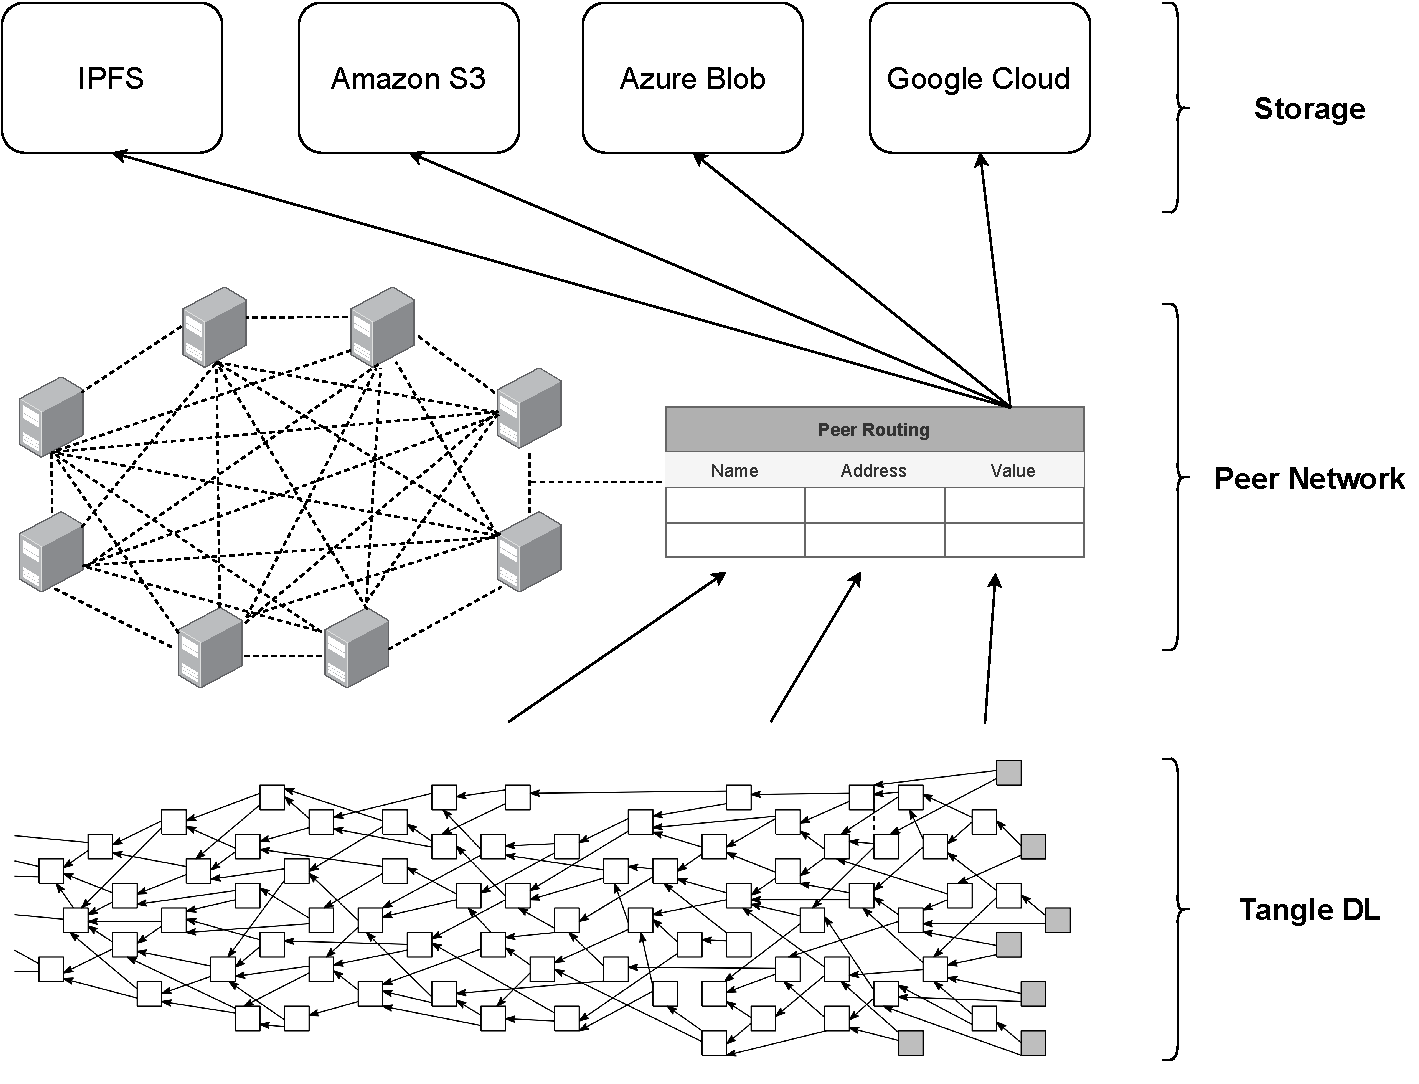
\includegraphics[width=0.8\textwidth,trim={0 0 0 0},clip]{figs/vivian_architecture.pdf}
    \caption{Vivian Architecture}
    \label{fig:vivian_architecture}
\end{figure*}

\subsection{Overview}
In designing Vivian, we want the system to achieve the following properties:

\begin{itemize}
    \item \textbf{Decentralized Naming and Look-up.} End-users can register for and bind values to human-meaningful names and look up the values of names without relying on the trust of central authorities.
    \item \textbf{Decentralized and Secure Storage.} End-users can store their data in a decentralized manner. In addition, users can control the access rights of their data.
    \item  \textbf{IoT Device Supported.} The whole processes like registering a name, looking up a name, and file handling should not be energy-hungry and hardware resource hungry.
          They can be accomplished by devices with limited hardware resources such as Raspberry Pi.
\end{itemize}

The overall architecture of Vivian can be divided into three layers: Tangle DL layer, Peer Network layer, and Storage layer.

\subsection{Naming System}

\subsection{Peer Network}

\subsection{Storage System}